%!TEX root = ../out/01-intro-SL.tex

\newcommand{\mycomp}[1]{\pgfmathparse{#1}\pgfmathprintnumber[precision=0]{\pgfmathresult}}

\begin{document}

\title[Introduction]
{Introduction to solving intractable problems}

\begin{frame}
	\titlepage{}
\end{frame}

\lecturenotes{\maketitle}

\begin{frame}
	\slides{\frametitle{Outline}}
	\tableofcontents
\end{frame}

\section{Algorithms for NP-hard problems}

\begin{frame}

	Central question
	\begin{center}
		{\huge $\P$ vs. $\NP$}
	\end{center}
\end{frame}

\begin{frame}
	\frametitle{NP-hard problems}

	\begin{itemize}
		\item no known polynomial time algorithm for any \NP-hard problem
		\item belief: $\P \neq \NP$
		      %  \item Exponential Time Hypothesis: 3-Sat cannot be solved in subexponential time
		      %  \item (thus many other problems cannot be solved in subexponential time either)
		\item What to do when facing an \NP-hard problem?
	\end{itemize}
\end{frame}


\begin{frame}
	\frametitle{Example problem}

	\begin{block}{Monitoring a power grid}
		Tammy is responsible for fault detection on the power grid of an energy company.\\\smallskip
		She has access to $k$ monitoring devices. Each one can be placed on a node of the electrical grid and can monitor the power lines that are connected to this node.\\\smallskip
		Tammy's objective is to place the monitoring devices in such a way that each power line is monitored by at least one monitoring device.
	\end{block}
	Let us first give an abstraction of this problem and formulate it as a decision problem for graphs.
\end{frame}


\begin{frame}{Example problem: \textsc{Vertex Cover}}

	\noindent
	A \alert{vertex cover} in a graph $G=(V,E)$ is a subset of vertices $S\subseteq V$ such that every edge of $G$ has an endpoint in $S$.

	\pbDefNoPara{\textsc{Vertex Cover}}{Graph $G$, integer $k$}{Does $G$ have a vertex cover of size $k$?}

	\noindent
	\textbf{Note:}
	\textsc{Vertex Cover} is \NP-complete.

	\begin{center}
		\begin{tikzpicture}[scale=0.7]
			\node[selected]  (a) at (1.5,3  ) {};
			\node[vertex] (b) at (3  ,3  ) {};
			\node[vertex] (c) at (0  ,1.5) {};
			\node[selected]                 (d) at (1.5,1.5) {};
			\node[selected]                 (e) at (3  ,1.5) {};
			\node[vertex] (f) at (1.5,0  ) {};
			\node[selected]                 (g) at (3  ,0  ) {};
			\node[vertex] (h) at (4.5,0  ) {};
			\draw[line width=1.5pt]     (a) -- (b) -- (e) -- (h) -- (g) -- (f) -- (d) -- (g) -- (e) -- (a) -- (c) -- (d) -- (a);
		\end{tikzpicture}
	\end{center}

\end{frame}



\begin{frame}{Coping with NP-hardness}
	\begin{itemize}
		\item Approximation algorithms
		      \begin{itemize}
			      \item There is a polynomial-time algorithm, which, given a graph $G$, finds a vertex cover of $G$ of size at most $2\cdot \OPT$, where $\OPT$ is the size of a smallest vertex cover of $G$.
		      \end{itemize}
		\item Exact exponential time algorithms
		      \begin{itemize}
			      \item There is an algorithm solving \textsc{Vertex Cover} in time $O(1.1970^n)$, where $n=|V|$~\cite{XiaoN17}.
		      \end{itemize}
		\item Fixed parameter algorithms
		      \begin{itemize}
			      \item There is an algorithm solving \textsc{Vertex Cover} in time $O(1.2738^k+kn)$~\cite{ChenKX10}.
		      \end{itemize}
		\item Heuristics
		      \begin{itemize}
			      \item The COVER heuristic (COVer Edges Randomly) finds a smaller vertex cover than state-of-the-art heuristics on a suite of hard benchmark instances~\cite{RichterHG07}.
		      \end{itemize}
		\item Restricting the inputs
		      \begin{itemize}
			      \item \textsc{Vertex Cover} can be solved in polynomial time on bipartite graphs, trees, interval graphs, etc.~\cite{Golumbic04}.
		      \end{itemize}
		\item Quantum algorithms?
		      \begin{itemize}
			      \item Not believed to solve \NP-hard problems in polynomial time~\cite{Aaronson05}. Quadratic speedup possible in some cases.
		      \end{itemize}
	\end{itemize}
\end{frame}

\begin{frame}{Aims of this course}

	\centering
	Design and analyze algorithms for \NP-hard problems.

	\bigskip

	\centering
	We focus on algorithms that solve \NP-hard problems \alert{exactly} and analyze their \alert{worst case running time}.
\end{frame}

\section{Exponential Time Algorithms}

\begin{frame}{Running times}

	Worst case running time of an algorithm.
	\begin{itemize}
		\item An algorithm is \alert{polynomial} if $\exists c\in \mathbb{N}$ such that the algorithm solves every instance in time $O(n^c)$, where $n$ is the size of the instance.\\
		      Also: $n^{O(1)}$ or $\poly(n)$.
		\item \alert{quasi-polynomial}: $2^{O(\log^c n)}$, $c\in O(1)$
		\item \alert{sub-exponential}: $2^{o(n)}$
		\item \alert{exponential}: $2^{\text{poly}(n)}$
		\item \alert{double-exponential}: $2^{2^{\text{poly}(n)}}$
	\end{itemize}

	\medskip
	$O^*$-notation ignores polynomial factors in the input size:
	\begin{align*}
		\cO^*(f(n)) & \equiv \cO(f(n) \cdot \mathsf{poly}(n)) \\
		\cO^*(f(k)) & \equiv \cO(f(k) \cdot \mathsf{poly}(n))
	\end{align*}

\end{frame}

\begin{frame}
	\frametitle{Brute-force algorithms for NP-hard problems}

	\begin{theorem}
		Every problem in \NP\ can be solved in exponential time.
	\end{theorem}
	\pause{}
	For a proof, see the lecture on \NP-completeness.
\end{frame}

\begin{frame}{Three main categories for NP-complete problems}
	\begin{itemize}
		\item Subset problems
		\item Permutation problems
		\item Partition problems
	\end{itemize}
\end{frame}

\begin{frame}
	\frametitle{Subset Problem: \textsc{Independent Set}}

	\noindent
	An \alert{independent set} in a graph $G=(V,E)$ is a subset of vertices $S\subseteq V$ such that the vertices in $S$ are pairwise non-adjacent in $G$.

	\pbDefNoPara{\textsc{Independent Set}}{Graph $G$, integer $k$}{Does $G$ have an independent set of size $k$?}

	\begin{center}
		\begin{tikzpicture}[scale=0.7]
			\node[vertex]  (a) at (1.5,3  ) {};
			\node[selected] (b) at (3  ,3  ) {};
			\node[selected] (c) at (0  ,1.5) {};
			\node[vertex]                 (d) at (1.5,1.5) {};
			\node[vertex]                 (e) at (3  ,1.5) {};
			\node[selected] (f) at (1.5,0  ) {};
			\node[vertex]                 (g) at (3  ,0  ) {};
			\node[selected] (h) at (4.5,0  ) {};
			\draw[line width=1.5pt]     (a) -- (b) -- (e) -- (h) -- (g) -- (f) -- (d) -- (g) -- (e) -- (a) -- (c) -- (d) -- (a);
		\end{tikzpicture}
	\end{center}

	\noindent
	Brute-force: \pause{}$O^*(2^n)$, where $n=|V(G)|$

\end{frame}


\begin{frame}
	\frametitle{Permutation Problem: \textsc{Traveling SalesPerson}}

	\pbDefNoPara{\textsc{Traveling SalesPerson} (TSP)}{a set of $n$ cities, the distance $d(i,j)\in \mathbb{N}$ between every two cities $i$ and $j$, integer $k$}{Is there a permutation of the cities (a \alert{tour}) such that the total distance when traveling from city to city in the specified order, and returning back to the origin, is at most $k$?}

	\begin{center}
		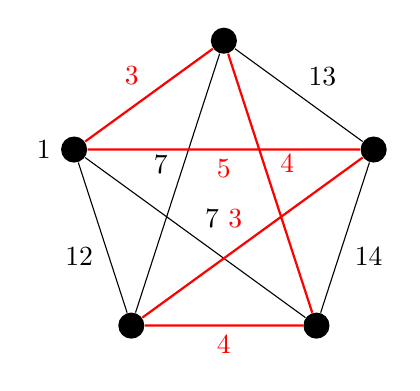
\begin{tikzpicture}
			\tikzstyle{vertex}=[minimum size=1mm,circle,color=black,fill=black]

			\draw ( 90:2cm) node[vertex] (5) {};
			\draw (162:2cm) node[vertex,label=left:$1$] (6) {};
			\draw (234:2cm) node[vertex] (7) {};
			\draw (306:2cm) node[vertex] (8) {};
			\draw ( 18:2cm) node[vertex] (9) {};

			\draw (5) to node[swap,auto] {$7$} (7)
			(5) to node[auto] {$13$} (9)
			(6) to node[swap,auto] {$12$} (7)
			(6) to node[auto] {$7$} (8)
			(8) to node[swap,auto] {$14$} (9);

			\draw[thick,red] (5) to node[swap,auto] {$3$} (6)
			(5) to node[auto] {$4$} (8)
			(6) to node[swap,auto] {$5$} (9)
			(7) to node[swap,auto] {$4$} (8)
			(7) to node[auto] {$3$} (9);
		\end{tikzpicture}
	\end{center}

	\noindent
	Brute-force: \pause{}$O^*(n!) \subseteq 2^{O(n \log n)}$

\end{frame}


\begin{frame}
	\frametitle{Partition Problem: \textsc{Coloring}}

	\noindent
	A \alert{$k$-coloring} of a graph $G=(V,E)$ is a function $f:V \rightarrow \{1,2, \ldots,k\}$ assigning colors to $V$ such that no two adjacent vertices receive the same color.

	\pbDefNoPara{\textsc{Coloring}}{Graph $G$, integer $k$}{Does $G$ have a $k$-coloring?}

	\begin{center}
		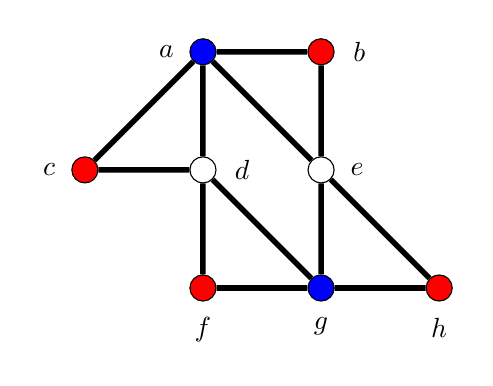
\begin{tikzpicture}
			\tikzstyle{vertex}=[minimum size=1mm,circle,draw,color=black,fill=black]
			\tikzstyle{every node}=[vertex]
			\node[vertex,fill=blue,label=left:$a$] (a) at (1.5,3  ) {};
			\node[vertex,fill=red,label=right:$b$]  (b) at (3  ,3  ) {};
			\node[vertex,fill=red,label=left:$c$]  (c) at (0  ,1.5) {};
			\node[vertex,fill=white,label=right:$d$](d) at (1.5,1.5) {};
			\node[vertex,fill=white,label=right:$e$](e) at (3  ,1.5) {};
			\node[vertex,fill=red,label=below:$f$]  (f) at (1.5,0  ) {};
			\node[vertex,fill=blue,label=below:$g$] (g) at (3  ,0  ) {};
			\node[vertex,fill=red,label=below:$h$]  (h) at (4.5,0  ) {};
			\draw[line width=2pt]     (a) -- (b) -- (e) -- (h) -- (g) -- (f) -- (d) -- (g) -- (e) -- (a) -- (c) -- (d) -- (a);
		\end{tikzpicture}
	\end{center}

	\noindent
	Brute-force: \pause{}$O^*(k^n)$, where $n=|V(G)|$

\end{frame}


\begin{frame}
	\frametitle{Exponential Time Algorithms}

	\begin{itemize}
		\item natural question in Algorithms:\\
		      design faster (worst-case analysis) algorithms for problems
		      \bigskip
		\item might lead to practical algorithms
		      \begin{itemize}
			      \item for small instances
			            \begin{itemize}
				            \item you don't want to design software where your client/boss can find with better solutions \emph{by hand} than your software
			            \end{itemize}
			      \item subroutines for
			            \begin{itemize}
				            \item (sub)exponential time approximation algorithms
				            \item randomized algorithms with expected polynomial run time
			            \end{itemize}
		      \end{itemize}
	\end{itemize}
\end{frame}


\begin{frame}
	\frametitle{Solve an NP-hard problem}

	\begin{itemize}
		\item exhaustive search
		      \begin{itemize}
			      \item trivial method
			      \item try all candidate solutions (certificates) for a ground set on $n$ elements
			      \item running times for problems in NP
			            \begin{itemize}
				            \item \textsc{Subset Problems}: $\cO^*(2^n)$
				            \item \textsc{Permutation Problems}: $\cO^*(n!)$
				            \item \textsc{Partition Problems}: $\cO^*(c^{n \log n})$
			            \end{itemize}
		      \end{itemize}
		\item faster exact algorithms
		      \begin{itemize}
			      \item for some problems, it is possible to obtain provably faster algorithms
			      \item running times $\cO(1.0836^n), \cO(1.4689^n), \cO(1.9977^n)$
		      \end{itemize}
	\end{itemize}
\end{frame}


\begin{frame}
	\frametitle{Exponential Time Algorithms in Practice}

	\begin{itemize}
		\item How large are the instances one can solve in practice?
	\end{itemize}

	\newcommand{\MIPS}{2^38}
	\pgfkeys{/pgf/fpu=true}
	\begin{center}\begin{tabular}{c  r r r r r}
			\toprule
			Available time                  & 1 s                                            & 1 min                           & 1 hour                           & 3 days                           & $6$ months\tabularnewline
			nb. of operations               & $2^{38}$                                       & $\sim 2^{44}$                   & $\sim 2^{50}$                    & $\sim 2^{56}$                    & $\sim 2^{62}$\tabularnewline
			\midrule
			$n^{5}$                         & \mycomp{\MIPS^(1/5)}                           & \mycomp{(2^6*\MIPS)^(1/5)}      & \mycomp{(2^12*\MIPS)^(1/5)}      & \mycomp{(2^18*\MIPS)^(1/5)}      & \mycomp{(2^24*\MIPS)^(1/5)}\tabularnewline
			$n^{10}$                        & \mycomp{\MIPS^(1/10)}                          & \mycomp{(2^6*\MIPS)^(1/10)}     & \mycomp{(2^12*\MIPS)^(1/10)}     & \mycomp{(2^18*\MIPS)^(1/10)}     & \mycomp{(2^24*\MIPS)^(1/10)}\tabularnewline
			$1.05^{n}$                      & \mycomp{ln(\MIPS)/ln(1.05)}                    & \mycomp{ln(2^6*\MIPS)/ln(1.05)} & \mycomp{ln(2^12*\MIPS)/ln(1.05)} & \mycomp{ln(2^18*\MIPS)/ln(1.05)} & \mycomp{ln(2^24*\MIPS)/ln(1.05)}\tabularnewline
			$1.1^{n}$                       & \mycomp{ln(\MIPS)/ln(1.1)}                     & \mycomp{ln(2^6*\MIPS)/ln(1.1)}  & \mycomp{ln(2^12*\MIPS)/ln(1.1)}  & \mycomp{ln(2^18*\MIPS)/ln(1.1)}  & \mycomp{ln(2^24*\MIPS)/ln(1.1)}\tabularnewline
			$1.5^{n}$                       &
			\mycomp{ln(     \MIPS)/ln(1.5)} &
			\mycomp{ln(2^6 *\MIPS)/ln(1.5)} &
			\mycomp{ln(2^12*\MIPS)/ln(1.5)} &
			\mycomp{ln(2^18*\MIPS)/ln(1.5)} & \mycomp{ln(2^24*\MIPS)/ln(1.5)}\tabularnewline
			$2^{n}$                         &
			\mycomp{ln(     \MIPS)/ln(2)}   &
			\mycomp{ln(2^6 *\MIPS)/ln(2)}   &
			\mycomp{ln(2^12*\MIPS)/ln(2)}   &
			\mycomp{ln(2^18*\MIPS)/ln(2)}   & \mycomp{ln(2^24*\MIPS)/ln(2)}\tabularnewline
			$5^{n}$                         &
			\mycomp{ln(     \MIPS)/ln(5)}   &
			\mycomp{ln(2^6 *\MIPS)/ln(5)}   &
			\mycomp{ln(2^12*\MIPS)/ln(5)}   &
			\mycomp{ln(2^18*\MIPS)/ln(5)}   & \mycomp{ln(2^24*\MIPS)/ln(5)}\tabularnewline
			$n!$                            &
			14                              &
			16                              &
			17                              &
			19                              &
			20\tabularnewline
			\bottomrule
		\end{tabular}\end{center}

	\medskip
	\textbf{Note:} Intel Core i7-8086K executes $\sim 2^{38}$ instructions per second at $5$ GHz.
\end{frame}


\begin{frame}

	\begin{quote}
		``For every polynomial-time algorithm you have, there is an exponential algorithm that I would rather run.''\\
		\flushright -- Alan Perlis (1922-1990, programming languages, 1st recipient of Turing Award)
	\end{quote}

\end{frame}


\begin{frame}
	\frametitle{Hardware vs. Algorithms}

	\begin{itemize}
		\item Suppose a $2^n$ algorithm enables us to solve instances up to size $x$
		\item Faster processors
		      \begin{itemize}
			      \item processor speed doubles after 18--24 months (Moore's law)
			      \item can solve instances up to size $x+1$
		      \end{itemize}
		\item Faster algorithm
		      \begin{itemize}
			      \item design an $O^*(2^{n/2}) \subseteq O(1.4143^{n})$ time algorithm
			      \item can solve instances up to size $2 \cdot x$
		      \end{itemize}
	\end{itemize}

\end{frame}


\section{Parameterized Complexity}


\begin{frame}
	\frametitle{A story}

	\noindent
	A computer scientist meets a biologist \ldots
	\slides{\vspace{6.5cm}}
	\lecturenotes{The biologist has performed $n$ experiments. Unfortunately, the data obtained from these experiments has some conflicts. He suspects that a small number $k$ of experiments have gone wrong, and he would like to detect whether removing $k$ experiments can solve all the conflicts.}

\end{frame}

\begin{frame}
	\frametitle{Eliminating conflicts from experiments}
	\noindent
	$n = 1000$ experiments,\\
	$k = 20$ experiments failed\\
	\bigskip

	\begin{center}
		\begin{tabular}{c c c}
			\toprule
			\multicolumn{3}{c}{Running Time}                                      \\
			Theoretical   & Number of Instructions & Real                         \\
			\midrule
			$2^n$         & $1.07 \cdot 10^{301}$  & $4.941 \cdot 10^{282}$ years \\
			$n^k$         & $10^{60}$              & $4.611 \cdot 10^{41}$  years \\
			$2^k \cdot n$ & $1.05 \cdot 10^9$      & $0.01526$ seconds            \\
			\bottomrule
		\end{tabular}
	\end{center}

	\bigskip
	\noindent
	Notes
	\begin{itemize}
		\item We assume that $2^{36}$ instructions are carried out per second.
		\item The Big Bang happened roughly $13.5\cdot 10^9$ years ago.
	\end{itemize}
\end{frame}

\begin{frame}
	\frametitle{Goal of Parameterized Complexity}

	\noindent
	Confine the combinatorial explosion to a parameter $k$.\\
	\bigskip

	\begin{center}
		
\includegraphics[height=2cm]{../img/pc.jpg}
	\end{center}

	\bigskip
	\noindent
	For which problem--parameter combinations can we find algorithms with running times of the form
	\begin{align*}
		f(k) \cdot n^{O(1)},
	\end{align*}
	where the $f$ is a computable function independent of the input size $n$?

\end{frame}


\begin{frame}
	\frametitle{Examples of Parameters}

	\pbDef{A Parameterized Problem}{an instance of the problem}{a parameter $k$}{a \Yes/\No{} question about the instance and the parameter}

	\slides{\bigskip}
	\begin{itemize}
		\item A parameter can be
		      \begin{itemize}
			      \item input size (trivial parameterization)
			      \item solution size
			      \item related to the structure of the input (maximum degree, treewidth, branchwidth, genus, \ldots)
			      \item etc.
		      \end{itemize}
	\end{itemize}

\end{frame}


\begin{frame}
	\frametitle{Main Complexity Classes}

	\noindent
	$\P$: class of problems that can be solved in time $n^{O(1)}$\newline
	$\FPT$: class of problems that can be solved in time $f(k) \cdot n^{O(1)}$\newline
	$\W[\cdot]$: parameterized intractability classes\newline
	$\XP$: class of problems that can be solved in time $f(k) \cdot n^{g(k)}$ %; ``polynomial when the parameter is a constant''.
	%
	\slides{\bigskip}
	\begin{align*}
		\P \subseteq \FPT \subseteq \W[1] \subseteq \W[2] \dots \subseteq \W[P] \subseteq \XP
	\end{align*}
	\slides{\bigskip}

	\noindent
	Known: If $\FPT = \W[1]$, then the Exponential Time Hypothesis fails,
	i.e. 3-\textsc{Sat} can be solved in time $2^{o(n)}$.

\end{frame}

\subsection{FPT Algorithm for Vertex Cover}

\begin{frame}
	\slides{\frametitle{Vertex Cover}}

	\pbDef{\textsc{Vertex Cover (VC)}}
	{A graph $G=(V,E)$ on $n$ vertices, an integer $k$}
	{$k$}
	{Is there a set of vertices $C \subseteq V$ of size at most $k$ such that every edge
		has at least one endpoint in $C$?}

	\begin{center}
		\begin{tikzpicture}[scale=1]

			\draw (0,0) node[selected] (v1) {};
			\draw (1,0) node[selected] (v2) {};
			\draw (2,0) node[vertex] (v3) {};
			\draw (3,0) node[selected] (v4) {};
			\draw (4,0) node[vertex] (v5) {};
			\draw (0,1) node[vertex] (v6) {};
			\draw (1,1) node[selected] (v7) {};
			\draw (3,1) node[vertex] (v8) {};
			\draw (4,1) node[selected] (v9) {};

			\draw[very thick] (v6)--(v1)--(v7)--(v8)--(v4)--(v5)--(v9) (v7)--(v2)--(v3);
			\draw[very thick] (v6)--(v7)--(v3) (v8)--(v9)--(v4);
		\end{tikzpicture}
	\end{center}

\end{frame}


\subsection{Algorithms for Vertex Cover}

\begin{frame}
	\frametitle{Brute Force Algorithms}

	\begin{itemize}
		\item $2^n \cdot n^{O(1)}$ not \FPT{}
		\item $n^k \cdot n^{O(1)}$ not \FPT{}
	\end{itemize}

\end{frame}


\begin{frame}
	\frametitle{An FPT Algorithm}

	\begin{algorithm}[H]
		\SetArgSty{}

		\alert{Algorithm $\text{vc1}(G,k)$}\;
		\BlankLine{}

		\lnl{algvctl:1}\If(\tcp*[f]{all edges are covered}){$E = \emptyset$} {
			\lnl{algvctl:2}\Return{Yes}
		}
		\lnl{algvctl:3}\ElseIf(\tcp*[f]{we cannot select any vertex}){$k \le 0$} {
			\lnl{algvctl:4}\Return{No}
		}
		\lnl{algvctl:5}\Else{
			\lnl{algvctl:6}Select an edge $uv\in E$\;
			\lnl{algvctl:7} \Return{$\text{vc1}(G - u, k-1) \;\vee\; \text{vc1}(G - v, k-1)$}
		}
	\end{algorithm}

\end{frame}

\begin{frame}{Running Time Analysis}
	\begin{itemize}
		\item Let us look at an arbitrary execution of the algorithm.
		\item Recursive calls form a \alert{search tree} $T$
		      \begin{itemize}
			      \item with depth $\le k$
			      \item where each node has $\le 2$ children
		      \end{itemize}
		\item $\Rightarrow$ $T$ has $\le 2^k$ leaves and $\le 2^{k}-1$ internal nodes
		\item at each node the algorithm spends time $n^{O(1)}$
		\item The running time is $O^*(2^k)$
	\end{itemize}
\end{frame}



\begin{frame}
	\frametitle{A faster FPT Algorithm}

	\pause{}

	\begin{algorithm}[H]
		\SetArgSty{}

		\alert{Algorithm $\text{vc2}(G,k)$}\;
		\BlankLine{}

		\lnl{algvctl2:1}\If(\tcp*[f]{all edges are covered}){$E = \emptyset$} {
			\lnl{algvctl2:2}\Return{Yes}
		}
		\lnl{algvctl2:3}\ElseIf(\tcp*[f]{we used too many vertices}){$k \le 0$} {
			\lnl{algvctl2:4}\Return{No}
		}
		\lnl{algvctl2:5}\ElseIf(\tcp*[f]{$G$ has maximum degree $\le 2$}){$\Delta(G) \le 2$} {
			\lnl{algvctl2:6}Solve the problem in polynomial time\;
		}
		\lnl{algvctl2:7}\Else{
		\lnl{algvctl2:8}Select a vertex $v$ of maximum degree\;
		\lnl{algvctl2:9} \Return{$\text{vc2}(G - v, k-1) \;\vee\; \text{vc2}(G - N[v], k-d(v))$}
		}
	\end{algorithm}

\end{frame}


\begin{frame}
	\frametitle{Running time analysis of vc2}

	\begin{itemize}
		\item Number of leaves of the search tree:
		      \begin{align*}
			      T(k) & \le T(k-1)+T(k-3)   \\
			      x^k  & \le x^{k-1}+x^{k-3} \\
			      x^3  & - x^2 - 1 \le 0
		      \end{align*}
		\item The equation $x^3 - x^2 - 1 = 0$ has a unique positive real solution: $x \approx 1.4655\ldots$
		\item Running time: $1.4656^k \cdot n^{O(1)}$
	\end{itemize}

\end{frame}

\section{Further Reading}

\begin{frame}
	\slides{\frametitle{Further Reading}}

	\begin{itemize}
		\item Exponential-time algorithms
		      \begin{itemize}
			      \item Chapter 1, \emph{Introduction}, in~\cite{FominK10}.
			      \item Survey on exponential-time algorithms~\cite{Woeginger01}.
			      \item Chapter 1, \emph{Introduction}, in~\cite{Gaspers10}.
		      \end{itemize}
		\item Parameterized Complexity
		      \begin{itemize}
			      \item Chapter 1, \emph{Introduction}, in~\cite{CyganFKL+15}
			      \item Chapter 2, \emph{The Basic Definitions}, in~\cite{DowneyF13}
			      \item Chapter I, \emph{Foundations}, in~\cite{Niedermeier06}
			      \item \emph{Preface} in~\cite{FlumG06}
		      \end{itemize}
	\end{itemize}

\end{frame}

\begin{frame}[t, allowframebreaks]
	\slides{\frametitle{References}}
	\printbibliography{}
\end{frame}

\end{document}
